%\documentclass[11pt,a4paper]{article}
\documentclass[11pt
  , a4paper
  , article
  , oneside
%  , twoside
%  , draft
]{memoir}

\usepackage{control}
\usepackage[numbers]{natbib}
\usepackage{tabulary}
%\usepackage{dhucs-ucshyper}
\usepackage{hyperref}


\begin{document}
 
\newcommand{\technumber}{
  RAON Control-Document Series\\
  Revision : v0.1,   Release : February. 15. 2016}
\title{\textbf{Git 사용자 매뉴얼}}

\author{박미정\thanks{mijoy0909@ibs.re.kr} {이상일\thanks{silee7103@ibs.re.kr}}\\
  Rare Isotope Science Project\\
  Institute for Basic Science, Daejeon, South Korea
}
\date{\today}


\renewcommand{\maketitlehooka}{\begin{flushright}\textsf{\technumber}\end{flushright}}
%\renewcommand{\maketitlehookb}{\centering\textsf{\subtitle}}
%\renewcommand{\maketitlehookc}{C}
%\renewcommand{\maketitlehookd}{D}

\maketitle

\begin{abstract}
본 문서는 제어그룹의 소스 코드 관리, 공유 및 협업을 위한 분산 버전 관리 시스템인 Git의 사용 방법을 설명한다\footnote{본 문서는 Debian Linux Jessie(64bit)/Windows 10(64bit) 환경에서 작성되었다.}.
\end{abstract}


\chapter{Git}
Git은 소프트웨어, 소스 코드 등의 변경 관리를 위한 분산 버전 관리 시스템으로 아래와 같은 특징을 가진다\footnote{Git Wikipedia, https://en.wikipedia.org/wiki/Git\_(software) (acessed Feb 17, 2016).}\footnote{Git 관련 용어 및 기초 지식은 Pro Git book, https://git-scm.com/book/ko/v2/을 참고바란다.}.

\begin{itemize}
	\item 효율적인 소스코드 버전 관리
	\item 프로젝트 공유 및 협업(병렬 개발) 가능
	\item 협업 과정에서 발생하는 이슈 트래킹 및 관리 용이
	\item 서버 저장소(Repository)의 문제 발생 시 로컬 저장소를 이용한 복원 가능
	\item 서버 저장소와 네트워크 접근에 대한 자유로움
\end{itemize}

\section{주요 명령어}
Git을 사용하기 위한 주요 명령어는 다음과 같다\footnote{Git - 간편안내서, https://rogerdudler.github.io/git-guide/index.ko.html (acessed Feb 16, 2016).}.

\begin{itemize}
	\item clone : git서버에 저장된 프로젝트 저장소를 로컬 저장소로 복제
	\item add : git에 작업 변경 사항(디렉토리, 파일의 생성 및 수정) 추가 
	\item rm : git에 존재하는 디렉토리, 파일 삭제 
	\item status : 작업중인 로컬 저장소 상태 확인
	\item commit : 상태 변화(추가, 삭제, 변경 등)에 대한 확정(로컬 저장소에 반영)
	\item push : 로컬 저장소에 반영된 사항을 서버 저장소로 반영
	\item pull : 서버 저장소의 변경사항 갱신
	\item log : commit에 관한 log 확인
	\item checkout : 로컬저장소 변경 내용 되돌리기 (변경 내용 및 생성 파일은 존재함)
	\item reset : 로컬저장소 변경 내용 초기화 (변경 내용 및 생성 파일 제거)
\end{itemize}

\chapter{GitLab}
Git은 RAON을 위해 내·외부에서 개발되는 장비별 소스 코드 등 소프트웨어의 체계적인 버전 관리 및 운영에 필수적이다. 이에 제어 그룹은 자체 서버에 설치형 Git인 GitLab을 설치하여 그림 \ref{fig:gitlab}과 같이 ‘RaonControl’이란 명을 가진 저장소(Repository)를 운영하고 있으며, GitLab에 대한 정보는 아래와 같다\footnote{게스트 계정은 공개된 프로젝트에 한해 git pull(내려받기) 가능하며, 계정 관련 문의(생성, 권한 요청 등) 및 기타 사항은 관리자(mijoy0909@ibs.re.kr)에게 연락 바란다.}.
\begin{itemize}
	\item 내부 접속 URL : http://10.1.5.12:30000 
	\item 외부 접속 URL : http://risp.synology.me:30000
	\item 게스트 계정 정보 :
	\begin{itemize}
		\item[*] Username : RISP
		\item[*] Password : risp1234
	\end{itemize}
	\item 공개 프로젝트 리스트 :
	\begin{itemize}
		\item[*] scripts\_for\_epics : EPICS 설치 및 환경구성 자동화 스크립트
		\item[*] siteLibs : EPICS IOC 개발 코드의 재사용을 위한 Library 구성 항목
		\item[*] siteApps : EPICS IOC 구성 항목
		\item[*] training : 제어그룹 내부 교육 자료
	\end{itemize}
\end{itemize}

\begin{figure}[!htb]
	\centering
	\subbottom[Control Group GitLab Page]
	{
		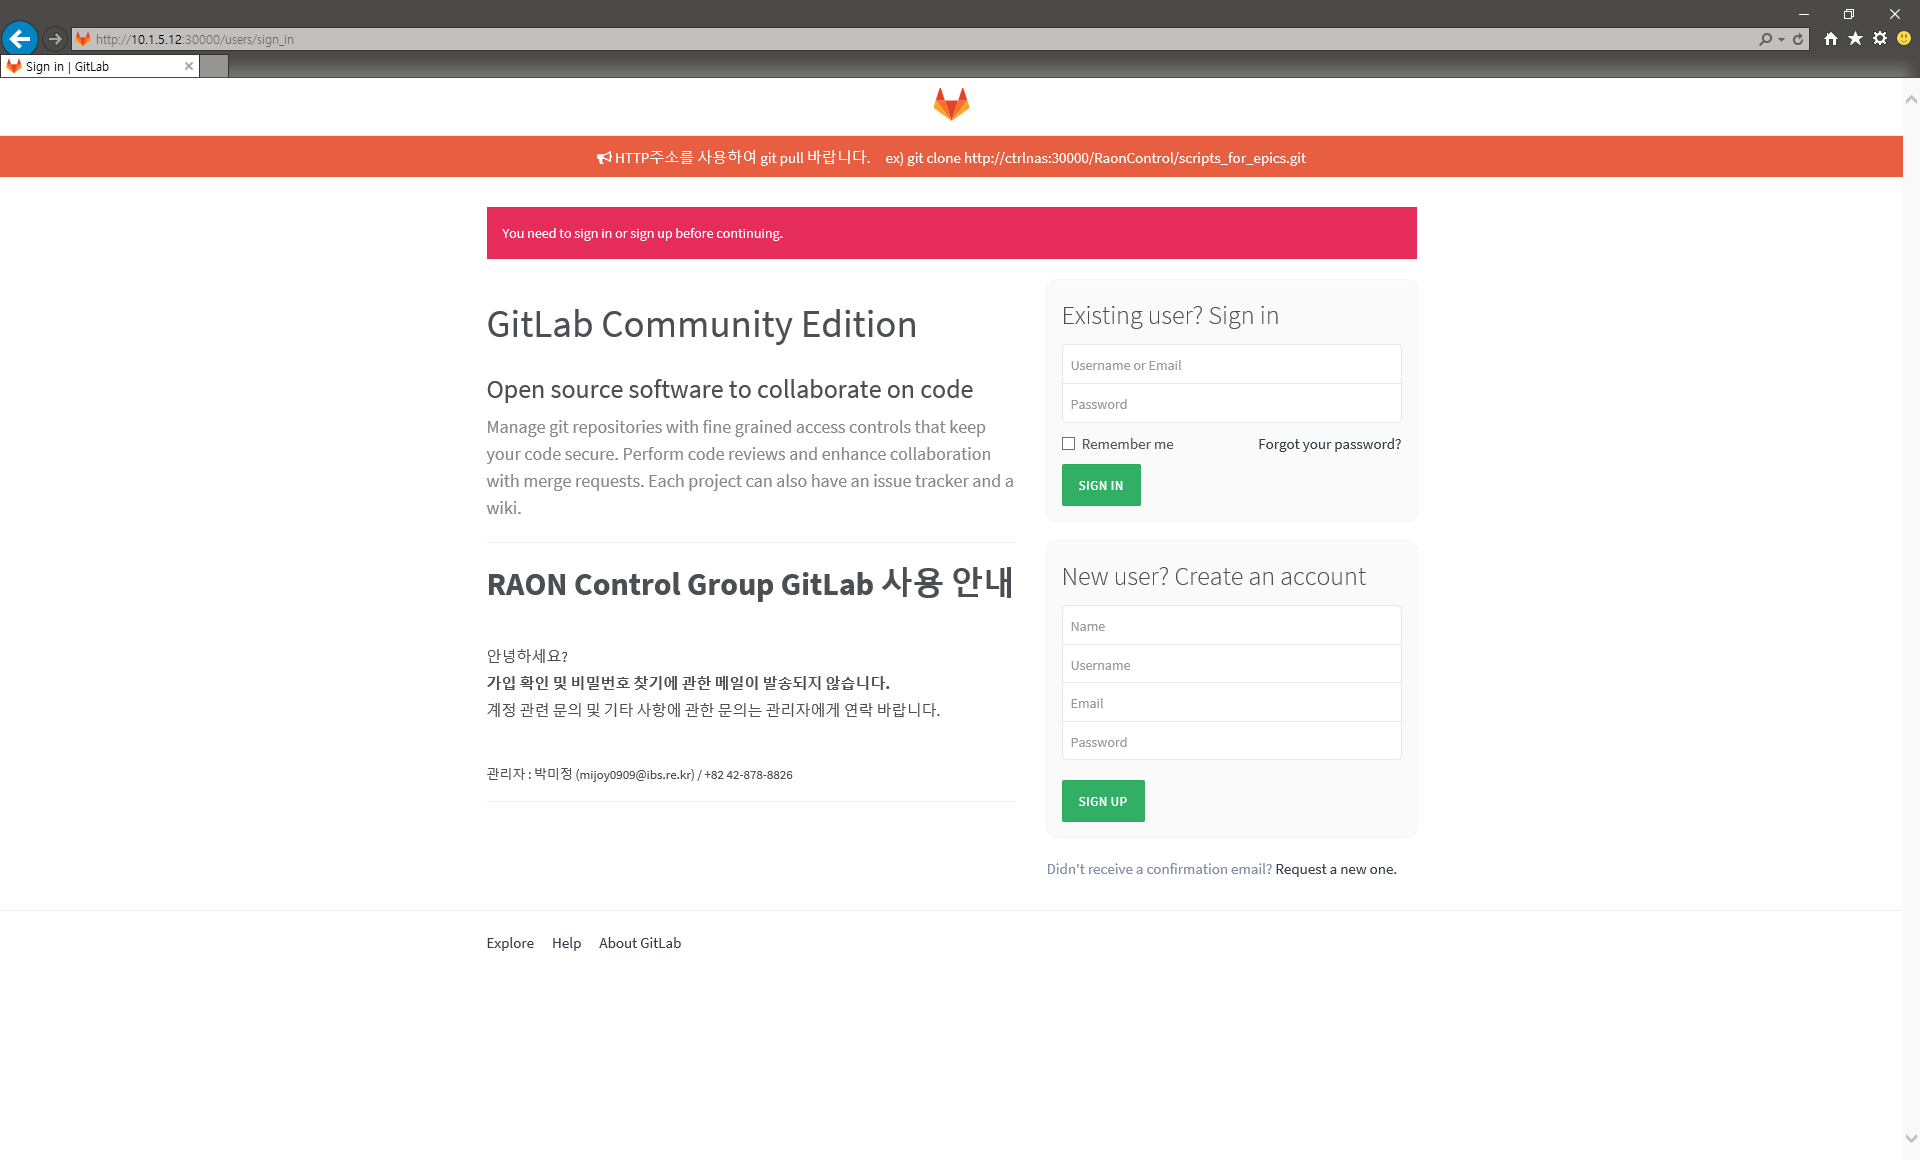
\includegraphics[width=0.99\textwidth]{./images/gitlab.PNG}
		\label{fig:gitlab1}     
	}
	\hfill
	\subbottom[Project Lists]
	{
		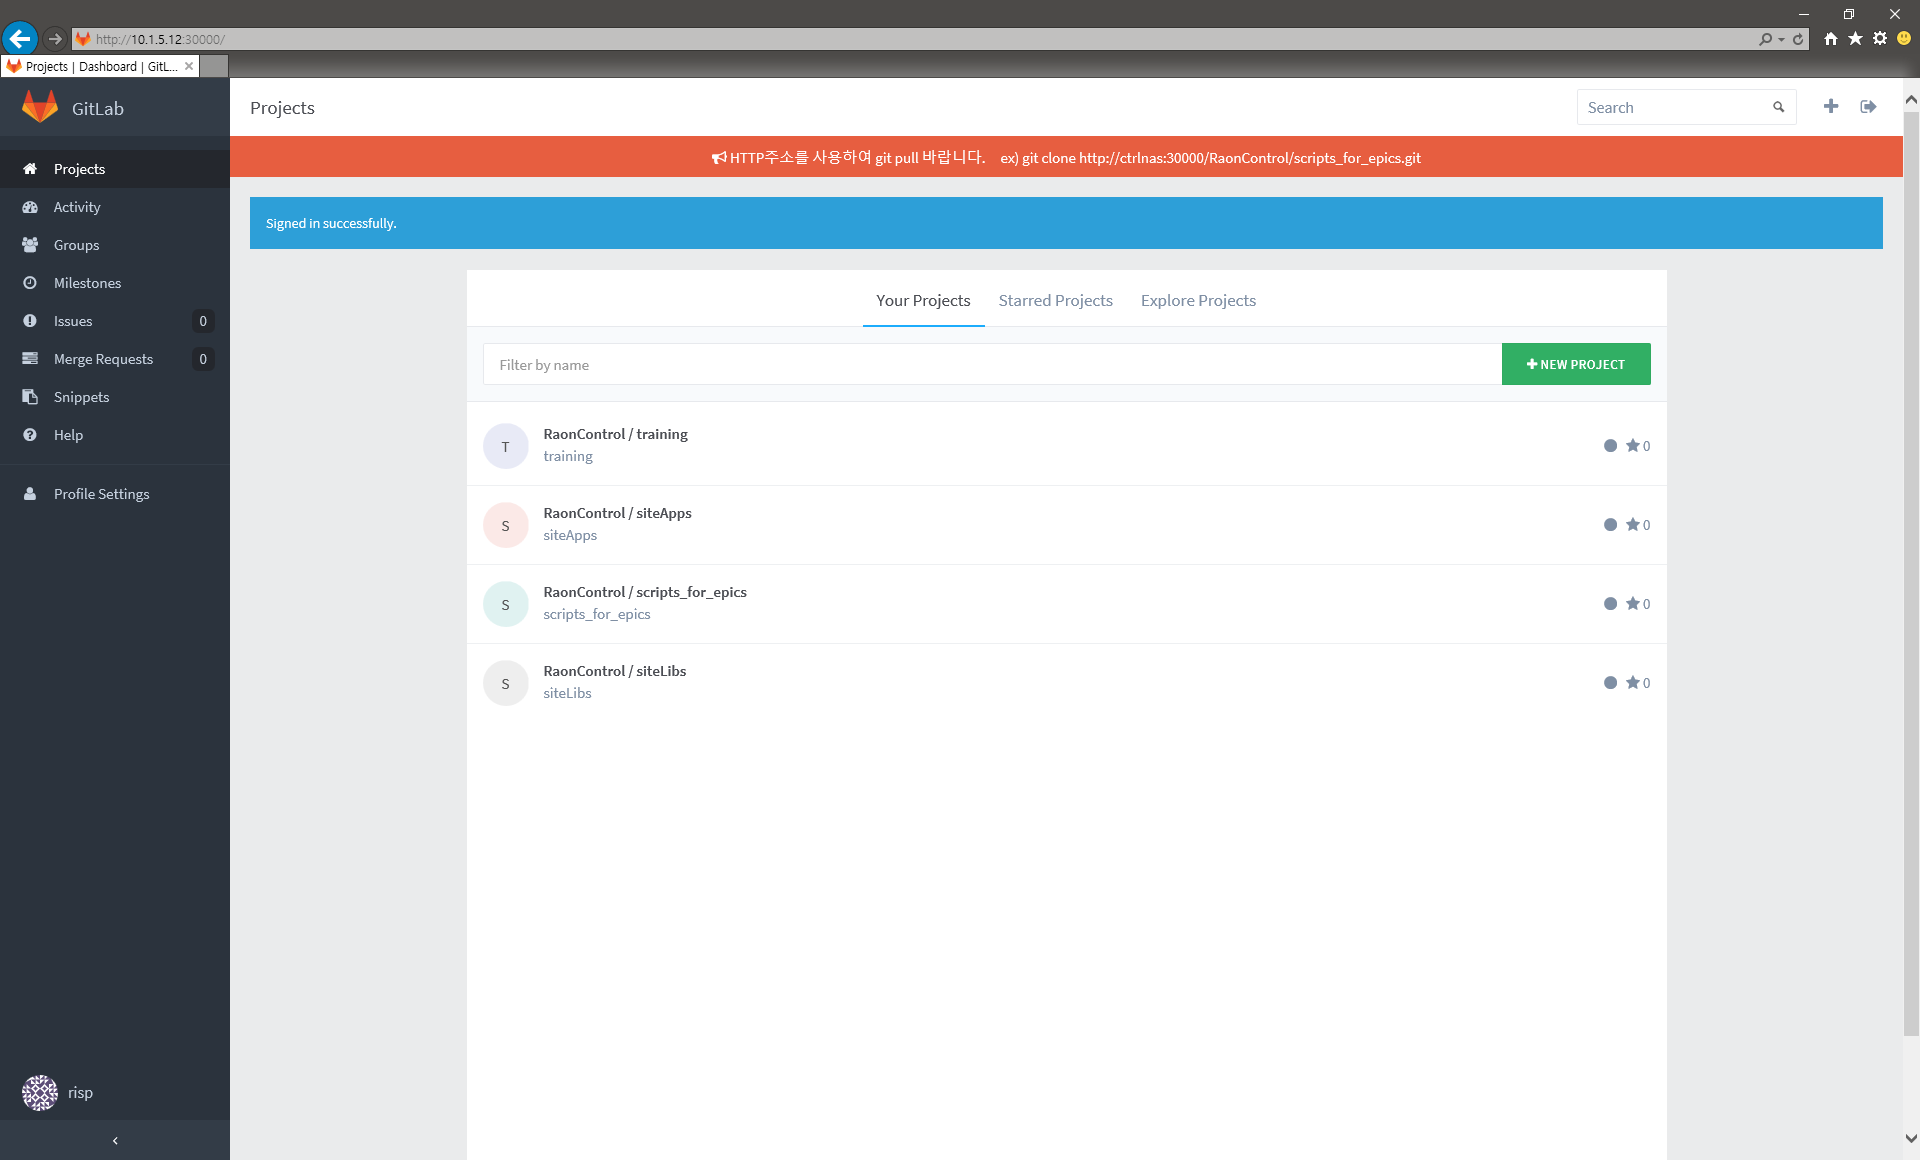
\includegraphics[width=0.99\textwidth]{./images/gitlab2.PNG}
		\label{fig:gitlab2}     
	}
	\caption{Control Group GitLab}
	\label{fig:gitlab}
\end{figure}
\clearpage

\section{Git 설치 및 기본 설정}
Git 사용에 앞서 본 문서는 안정적인 자동화 설치 스크립트 사용 및 EPICS IOC 개발을 위해 아래의 운영체제 사용을 권장한다.
\begin{itemize}
	\item Debian Linux 계열 (Whizzy, Jessie) 32bit/64bit
	\item Ubuntu Linux 32bit/64bit
\end{itemize}

\subsection{설치 방법}
\subsubsection{- Linux}
Git 사용을 위해서는 Git Package 및 의존성을 가지는 라이브러리의 설치가 요구되며, 설치 방법은 아래와 같다.

\begin{itemize}
\item Debian / Ubuntu 계열 
	\begin{lstlisting}[style=termstyle]	
	mijoy0909@mjpark:~$ su
	Password: 
	root@mjpark:/home/mijoy0909# 
	root@mjpark:/home/mijoy0909# aptitude install git	\end{lstlisting}	 
\end{itemize}

\subsubsection{- Windows}
만약 리눅스 운영체제 사용이 불가피한 경우 Windows System에서 Git 사용 환경 구성을 위해서는 윈도우용 Git 프로그램인 msysgit(이하 Git)이 필요하다. 이는 그림 \ref{fig:gitinstall1}의 Git 웹페이지\href{http://git-scm.com/download/win}{(바로가기)}에서 다운 받을 수 있다\footnote{Windows용 Git 다운로드 페이지, http://git-scm.com/download/win.}\footnote{본 문서는 Git 2.7.1.2 버전을 사용하였다.}.

\begin{figure}[h!]
	\centering
	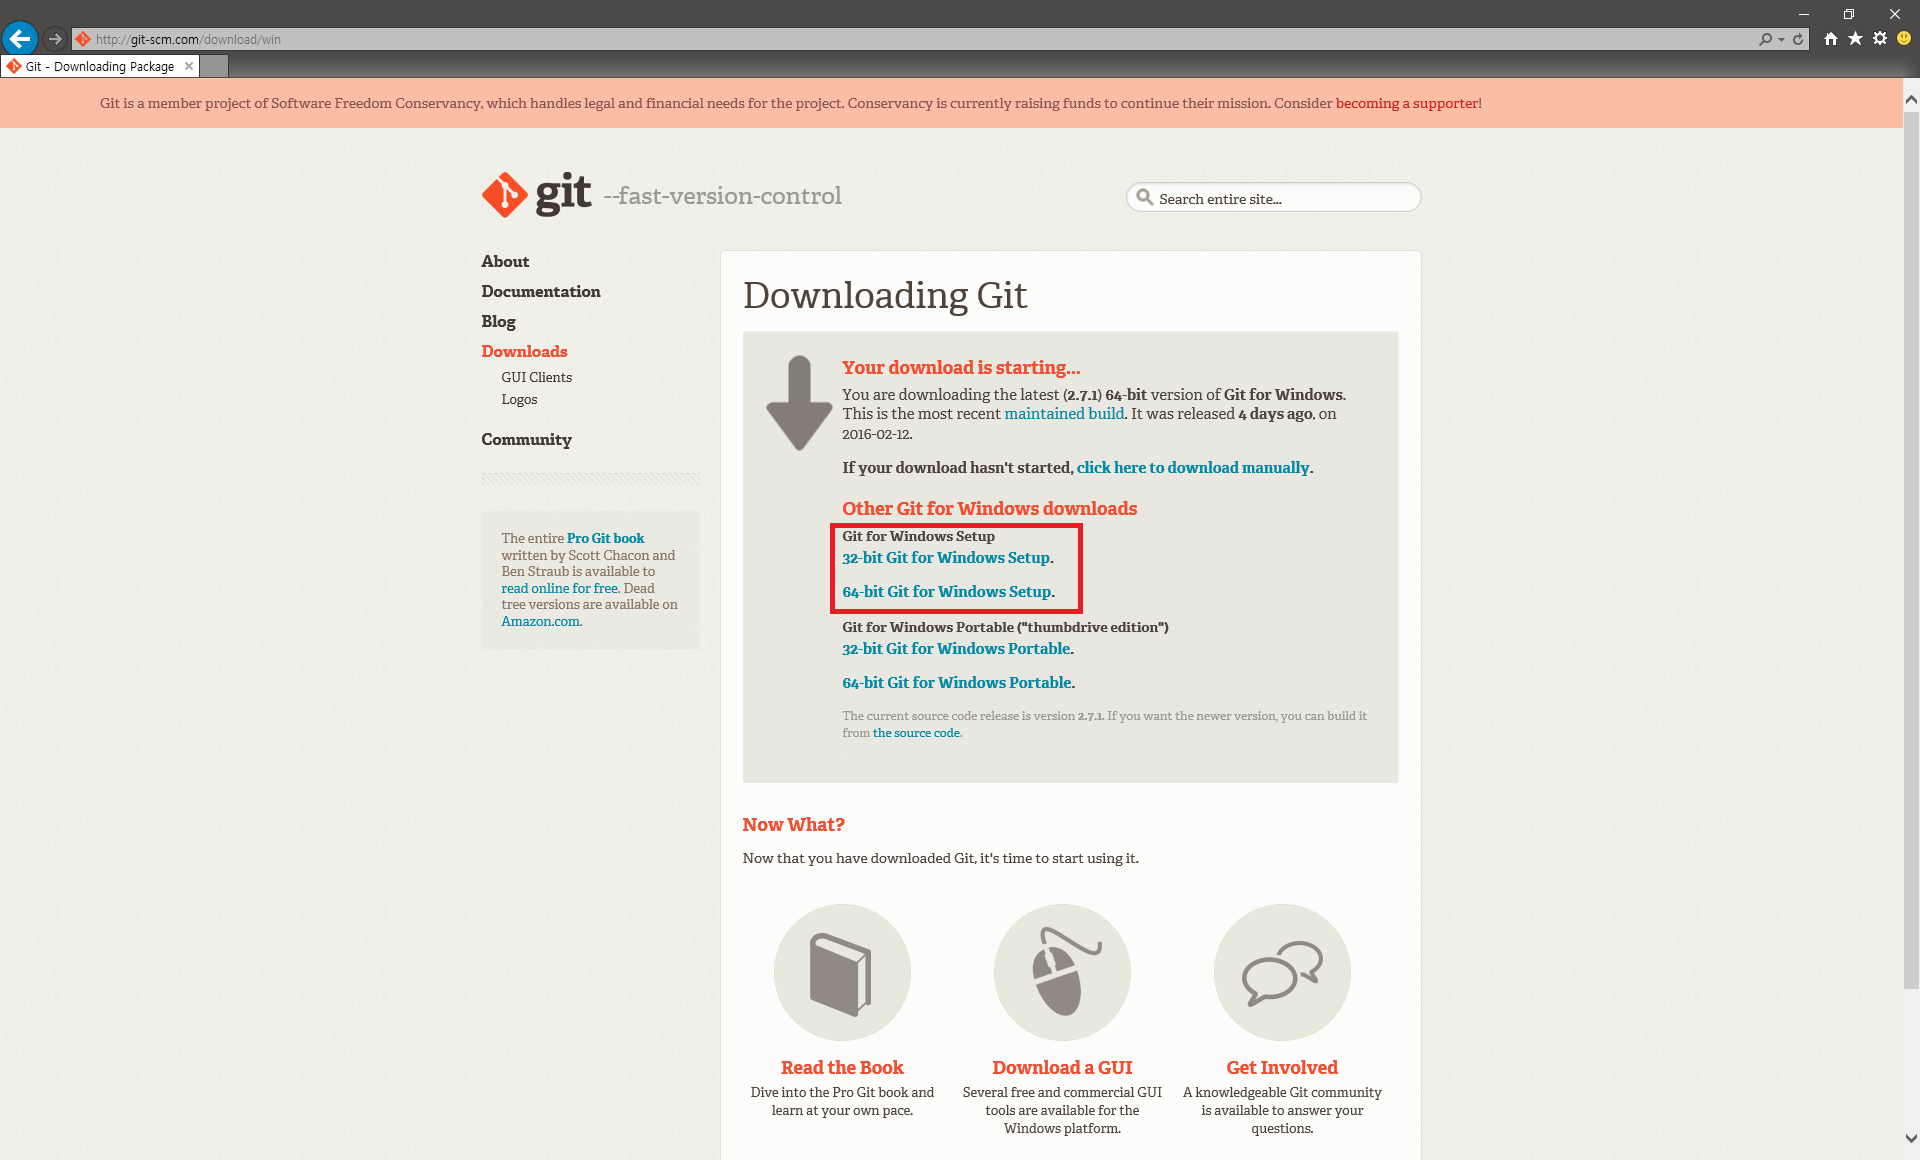
\includegraphics[width=0.71\textwidth]{./images/gitinstall1.PNG}
	\caption{Git (msysgit) Download Page}
	\label{fig:gitinstall1}
\end{figure}

\clearpage

\begin{itemize}
	\item Git 설치 (v2.7.1.2)\\
	다운로드한 Git을 아래의 절차로 설치한다.
	\begin{figure}[!htb]
		\centering
		\subbottom 
		{
			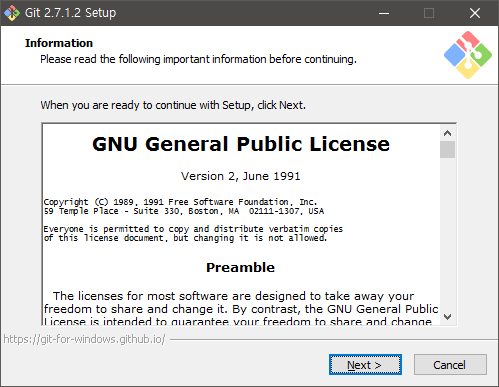
\includegraphics[width=0.5\textwidth]{./images/gitinstall2.PNG}%
			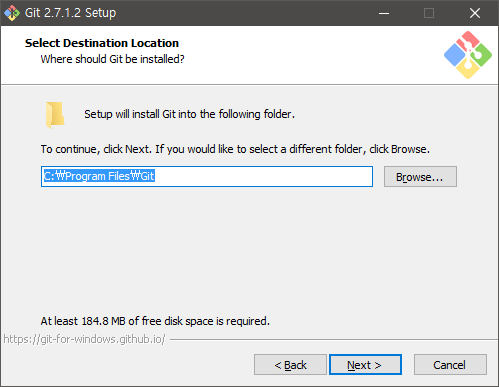
\includegraphics[width=0.5\textwidth]{./images/gitinstall3.PNG}
		}
		\subbottom
		{
			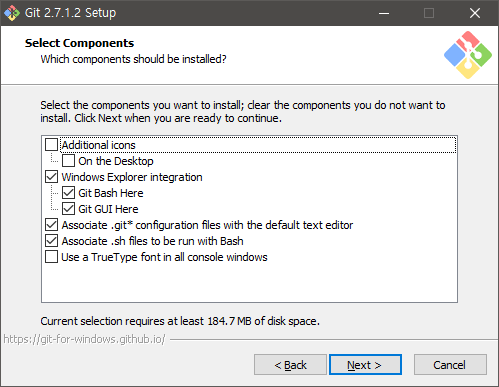
\includegraphics[width=0.5\textwidth]{./images/gitinstall4.PNG}%
			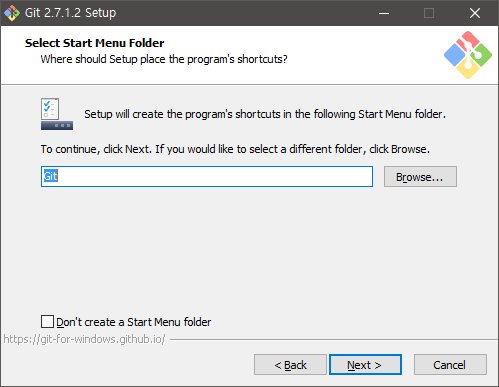
\includegraphics[width=0.5\textwidth]{./images/gitinstall5.PNG}   
		}
		\subbottom
		{
			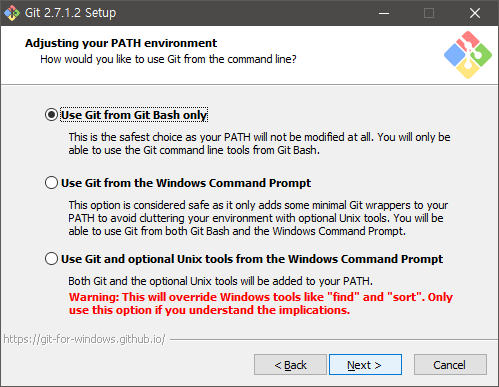
\includegraphics[width=0.5\textwidth]{./images/gitinstall6.PNG}%
			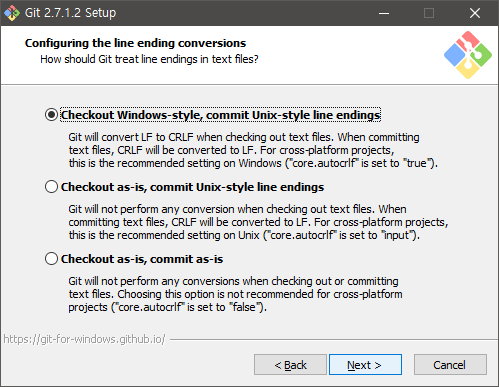
\includegraphics[width=0.5\textwidth]{./images/gitinstall7.PNG}   
		}
	\end{figure}	
	\clearpage
	\begin{figure}[!htb]
		\centering	
		\subbottom
		{
			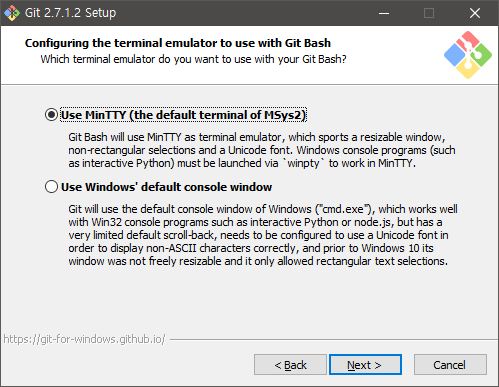
\includegraphics[width=0.5\textwidth]{./images/gitinstall8.PNG}%
			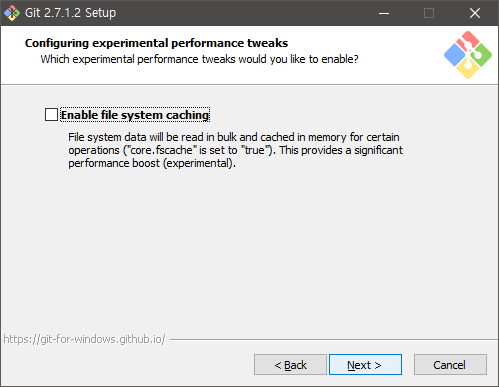
\includegraphics[width=0.5\textwidth]{./images/gitinstall9.PNG}   
		}
		\subbottom
		{
			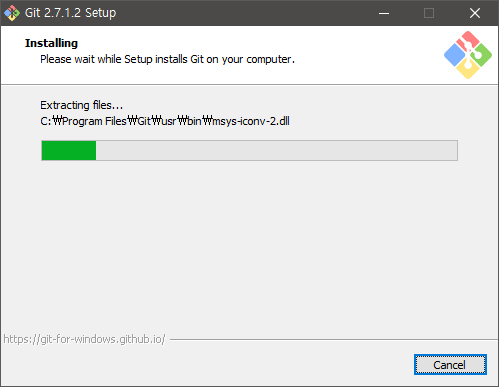
\includegraphics[width=0.5\textwidth]{./images/gitinstall10.PNG}%
			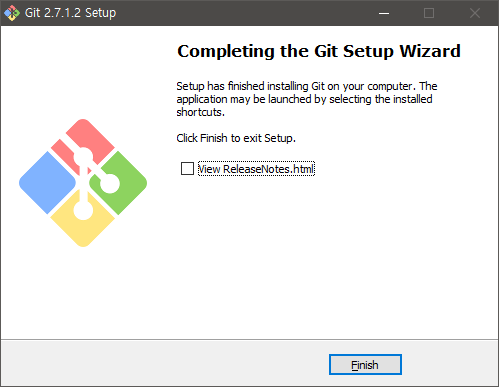
\includegraphics[width=0.5\textwidth]{./images/gitinstall11.PNG}   
		}			
		\caption{Windows Git v2.7.1.2 설치 과정}
	\end{figure}
	
\clearpage

	\item CLI 사용\\
	Git 설치 후 그림 \ref{fig:gitinstall12}와 같이 작업 할 폴더에서 마우스 오른쪽 버튼 클릭 후 ‘Git Bash Here’을 클릭하면 Windows에서 Git 사용을 위해 CLI (Command Line Interface)를 사용할 수 있다.	
		\begin{figure}[h!]
		\centering
		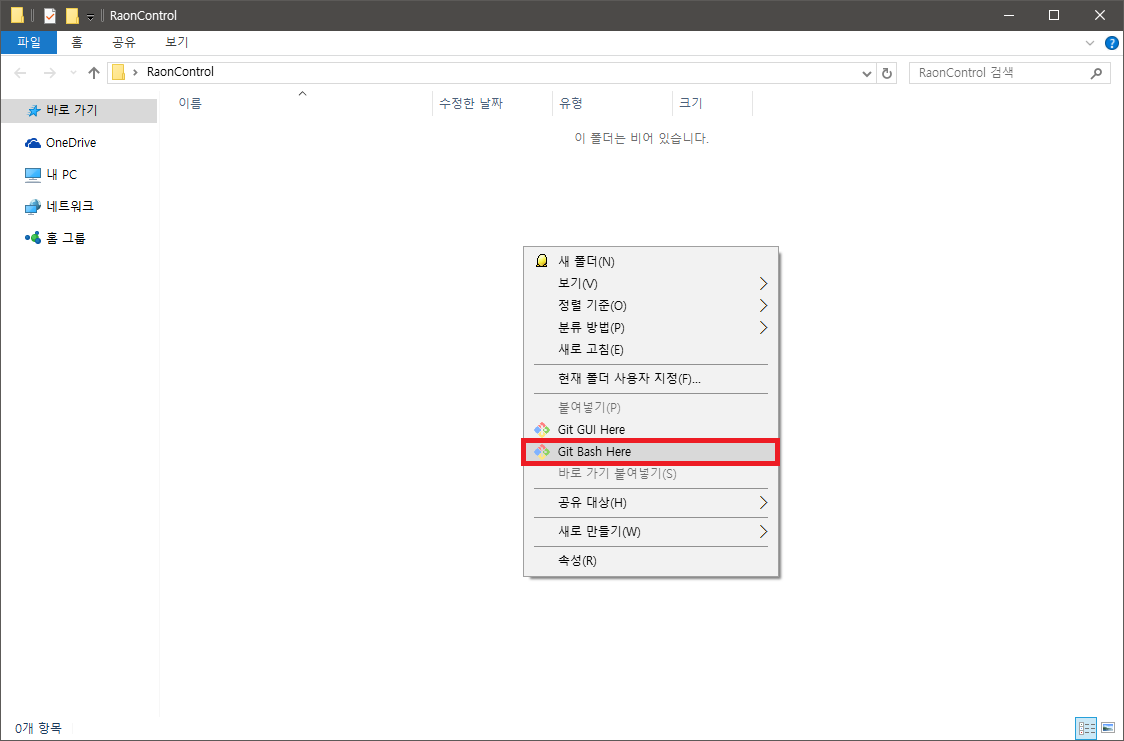
\includegraphics[width=0.85\textwidth]{./images/gitinstall12.PNG}
		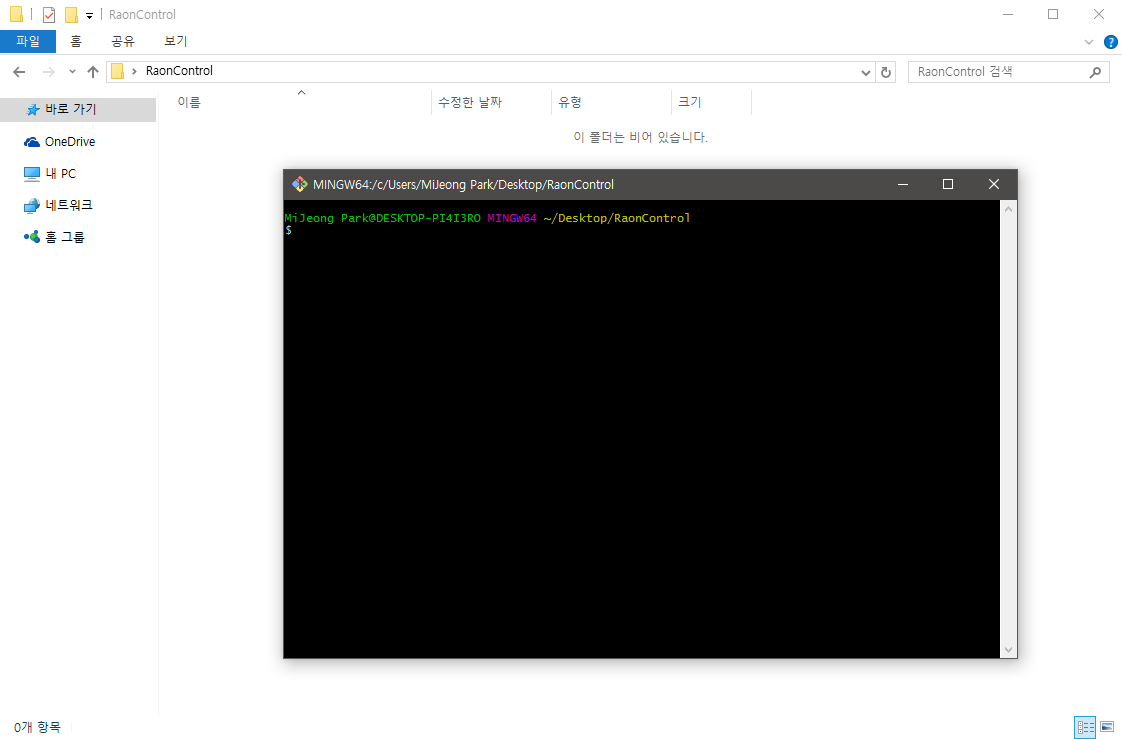
\includegraphics[width=0.85\textwidth]{./images/gitinstall12-1.PNG}
		\caption{Git Bash Shell 열기}
		\label{fig:gitinstall12}
		\end{figure}		
\end{itemize}

\subsection{기본 설정}
Git 사용에 앞서 설정해야하는 기본 사항 및 관련 명령어는 아래와 같다. 
\subsubsection{- 사용자 정보}
\small\textbf{이 설정은 commit 로그에서 작업자 확인을 위해 필수로 설정해야 한다.}	\begin{lstlisting}[style=termstyle, escapechar=!]	
	git config --global user.name "UserName" 
	git config --global user.email "Email Address" \end{lstlisting}
	
\begin{lstlisting}[style=termstyle, escapechar=!]
	mijoy0909@mjpark:~/RaonControl$ !\color{codegreen}{git config --global user.name "MiJeong Park"}!
	mijoy0909@mjpark:~/RaonControl$ !\color{codegreen}{git config --global user.email "mijoy0909@ibs.re.kr"}! \end{lstlisting}

\subsubsection{- 편집기}
	commit 등에 사용할 Git 텍스트 편집기를 설정한다. 기본적으로 Git은 Vi, Vim을 지원한다\footnote{Vi/Vim 사용은 vi 주요 단축키 Wiki Page, http://zetawiki.com/wiki/Vi\_주요\_단축키를 참고바란다.}. 하지만 Emacs 등의 다른 편집기 사용 시 아래와 같이 설정할 수 있다.
	\begin{lstlisting}[style=termstyle, escapechar=!]	
	git config --global core.editor emacs" \end{lstlisting}

\subsubsection{- 설정 확인}
Git 사용을 위해 설정된 환경을 확인한다.
	\begin{lstlisting}[style=termstyle, escapechar=!]	
	git config --list \end{lstlisting}

\section{Git 사용 방법}
\subsection{서버 저장소에서 로컬 저장소로 프로젝트 복제 : clone}
서버 저장소에서 작업하고자하는 로컬 저장소로 프로젝트를 복제하는 방법은 아래와 같다. Windows 운영체제는 팝업창에서 Username과 Password를 입력한다.

	\begin{lstlisting}[style=termstyle, escapechar=!]	
	git clone http://10.1.5.12:30000/RaonControl/ProjectName.git \end{lstlisting}
	
	\begin{lstlisting}[style=termstyle, escapechar=!]	
	mijoy0909@mjpark:~/RaonControl$ ls
	mijoy0909@mjpark:~/RaonControl$ 
	mijoy0909@mjpark:~/RaonControl$ !\color{codegreen}{git clone http://10.1.5.12:30000/RaonControl/training.git}!
	Cloning into 'training'...
	Username for 'http://10.1.5.12:30000': mijoy  
	Password for 'http://mijoy@10.1.5.12:30000': 
	remote: Counting objects: 105, done.
	remote: Compressing objects: 100% (80/80), done.
	remote: Total 105 (delta 18), reused 105 (delta 18)
	Receiving objects: 100% (105/105), 18.84 MiB | 0 bytes/s, done.
	Resolving deltas: 100% (18/18), done.
	Checking connectivity... done. 
	mijoy0909@mjpark:~/RaonControl$ ls
	training
	mijoy0909@mjpark:~/RaonControl$ cd training/
	mijoy0909@mjpark:~/RaonControl/training$ ls
	README.md  Tr1  Tr2  Tr3  Tr4 \end{lstlisting}
	
\subsection{새로운 디렉토리, 파일 생성 및 기존 파일 수정 : status, add, commit}

	\subsubsection {1. 변경 사항 확인}
	\begin{lstlisting}[style=termstyle, escapechar=!]	
	mijoy0909@mjpark:~/RaonControl/training$ !\color{codegreen}{git status}!                      
	On branch master
	Your branch is up-to-date with 'origin/master'.
	Changes not staged for commit:
	(use "git add <file>..." to update what will be committed)
	(use "git checkout -- <file>..." to discard changes in working directory)
	
         modified:   README.md
	
	Untracked files:
	(use "git add <file>..." to include in what will be committed)
	
	      TEMP/
	
	no changes added to commit (use "git add" and/or "git commit -a") \end{lstlisting}

	\subsubsection {2. 변경 사항 추가}
	\begin{lstlisting}[style=termstyle, escapechar=!]	
	mijoy0909@mjpark:~/RaonControl/training$  !\color{codegreen}{git add README.md TEMP/}! or !\color{codegreen}{git add .}!
	mijoy0909@mjpark:~/RaonControl/training$  !\color{codegreen}{git status}!
	On branch master
	Your branch is up-to-date with 'origin/master'.
	Changes to be committed:
	(use "git reset HEAD <file>..." to unstage)

	     modified:   README.md
	     new file:   TEMP/test.md
	     new file:   TEMP/test/test
	     new file:   TEMP/test/test.c \end{lstlisting}
	
	\subsubsection {3. 변경 사항 로컬 저장소에 반영}
	\begin{lstlisting}[style=termstyle, escapechar=!] 
	git commit -m "log message" \end{lstlisting}
	
	\begin{lstlisting}[style=termstyle, escapechar=!]	
	mijoy0909@mjpark:~/RaonControl/training$  !\color{codegreen}{git commit -m "modified README.md \& add TEMP (This is}!
	!\color{codegreen}{ test.)"}!
	[master 11182f9] modified README.md & add TEMP (This is test.)
	 4 files changed, 7 insertions(+), 2 deletions(-)
	 create mode 100644 TEMP/test.md
	 create mode 100755 TEMP/test/test
	 create mode 100644 TEMP/test/test.c \end{lstlisting}

	\subsubsection {4. 변경 사항 서버 저장소에 반영}
	\begin{lstlisting}[style=termstyle, escapechar=!]	
	mijoy0909@mjpark:~/RaonControl/training$  !\color{codegreen}{git push}! 
	Username for 'http://10.1.5.12:30000': mijoy
	Password for 'http://mijoy@10.1.5.12:30000': 
	Counting objects: 8, done.
	Delta compression using up to 2 threads.
	Compressing objects: 100% (7/7), done.
	Writing objects: 100% (8/8), 2.91 KiB | 0 bytes/s, done.
	Total 8 (delta 1), reused 0 (delta 0)
	To http://10.1.5.12:30000/RaonControl/training.git
	   53f825f..11182f9  master -> master
	mijoy0909@mjpark:~/RaonControl/training$ \end{lstlisting}	
	\clearpage
	\subsubsection {5. Commit Log 확인}
	\begin{lstlisting}[style=termstyle, escapechar=!]	
	mijoy0909@mjpark:~/RaonControl/training$ !\color{codegreen}{git log}!
	commit 11182f953f4d0a5f715b1a9cfad40f65193def1c
	Author: MiJeong Park <mijoy0909@ibs.re.kr>
	Date:   Thu Feb 18 14:35:52 2016 +0900
	
    	modified README.md & add TEMP (This is test.) \end{lstlisting}	

\vspace{5mm}
\subsection{서버 저장소의 최신 버전으로 갱신 : pull}
Git은 각자의 로컬 저장소에서 작업을 수행하기 때문에 다른 사람의 로컬 저장소에서 변경된 사항을 자신의 로컬 저장소로 갱신이 필요하다. 즉, 서버 저장소에 반영된 최신 버전의 프로젝트를 자신의 로컬 저장소로 업데이트하는 방법은 아래와 같다. 

	\begin{lstlisting}[style=termstyle, escapechar=!]	
	mijoy0909@mjpark:~/RaonControl/training$ !\color{codegreen}{git pull}!
	Username for 'http://10.1.5.12:30000': mijoy
	Password for 'http://mijoy@10.1.5.12:30000': 
	remote: Counting objects: 3, done.
	remote: Compressing objects: 100% (2/2), done.
	remote: Total 3 (delta 1), reused 0 (delta 0)
	Unpacking objects: 100% (3/3), done.
	From http://10.1.5.12:30000/RaonControl/training
    	702a2da..36001c4  master     -> origin/master
	Updating 702a2da..36001c4
	Fast-forward
	 TEMP.md | 2 +-
	 1 file changed, 1 insertion(+), 1 deletion(-)
	mijoy0909@mjpark:~/RaonControl/training$ $  \end{lstlisting}		

\subsection{EPICS IOC 개발 코드 형상관리}
Software 개발 코드 및 운영을 위한 형상관리를 위하여 통일된 개발 및 운영환경을 유지하기 위하여 다음과 같은 환경을 구성한다. 아래 디렉토리 구조는 "EPICS 자동화 설치 가이드라인"을 통하여 설치한 화면이다.

\subsubsection {1. git pull: siteLibs/siteApps, extLibs/extApps}
	siteLibs: IOC 구성을 위해 재사용 가능한 Software Library 
	\begin{lstlisting}[style=termstyle, escapechar=!]	
    ctrluser@silee:~/epics/R3.14.12.5$ !\color{codegreen}git clone http://10.1.5.12:30000/RaonControl/siteLibs.git!
    Cloning into 'siteLibs'...
    Username for 'http://10.1.5.12:30000': !\color{codegreen}silee7103!
    Password for 'http://silee7103@10.1.5.12:30000': 
    remote: Counting objects: 499, done.
    remote: Compressing objects: 100% (374/374), done.
    remote: Total 499 (delta 81), reused 499 (delta 81)
    Receiving objects: 100% (499/499), 1.58 MiB | 0 bytes/s, done.
    Resolving deltas: 100% (81/81), done.
    Checking connectivity... done.
    \end{lstlisting}		
    siteApps: IOC 개발 및 운영될 디렉토리
    \begin{lstlisting}[style=termstyle, escapechar=!]	
    ctrluser@silee:~/epics/R3.14.12.5$ !\color{codegreen}git clone http://10.1.5.12:30000/RaonControl/siteApps.git!
    Cloning into 'siteApps'...
    Username for 'http://10.1.5.12:30000': !\color{codegreen}silee7103!
    Password for 'http://silee7103@10.1.5.12:30000': 
    remote: Counting objects: 1422, done.
    remote: Compressing objects: 100% (946/946), done.
    remote: Total 1422 (delta 431), reused 1397 (delta 418)
    Receiving objects: 100% (1422/1422), 10.75 MiB | 11.20 MiB/s, done.
    Resolving deltas: 100% (431/431), done.
    Checking connectivity... done.
    \end{lstlisting}
    extLibs: IOC 구성을 위해 재사용 가능한 Software Library(외부 개발 코드)
    \begin{lstlisting}[style=termstyle, escapechar=!]	
    ctrluser@silee:~/epics/R3.14.12.5$ !\color{codegreen}git clone http://10.1.5.12:30000/RaonControl/extLibs.git!
    Cloning into 'siteLibs'...
    Username for 'http://10.1.5.12:30000': !\color{codegreen}silee7103!
    Password for 'http://silee7103@10.1.5.12:30000': 
    Checking connectivity... done.
    \end{lstlisting}		
    extApps: IOC 개발 및 운영될 디렉토리
    \begin{lstlisting}[style=termstyle, escapechar=!]	
    ctrluser@silee:~/epics/R3.14.12.5$ !\color{codegreen}git clone http://10.1.5.12:30000/RaonControl/extApps.git!
    Cloning into 'siteApps'...
    Username for 'http://10.1.5.12:30000': !\color{codegreen}silee7103!
    Password for 'http://silee7103@10.1.5.12:30000': 
    Checking connectivity... done.
    \end{lstlisting}

	\subsubsection {2. 개발디렉토리 구조}
	base: EPICS 구성을 위한 필수 항목 (통신, DB, Channel Access 관련 필수항목)\\
	epicsLibs: EPICS syncApp을 구성하기 위한 항목 \\
	extensions: EPICS (base외에 추가적인 항목, StripChart, gateway, 등) \\
	setEpicsEnv.sh: EPICS 개발 및 운영을 위한 환경변수 모음 \\
	\\
	siteLibs: RAON에 종속적인 EPICS IOC 개발관련 라이브러리 \\
	siteApps: RAON EPICS IOC 개발 및 운영 \\
	extLibs: 외부 개발 업체에서 개발되는 라이브러리 코드 모음 폴더 \\
	extApps: 오부 개발 업체 EPICS IOC 개발 및 운영 폴더 \\
	
	extLibs/extApps는 외부 개발 업체로 부터 개발된 코드 및 운영환경에 대한 형상관리를 위한다. 여기서 검증된 Software에 대한 부분은 향 후 siteLibs/siteApps에서 포함 시켜 관리한다.
	
	\begin{lstlisting}[style=termstyle, escapechar=!]
	ctrluser@silee:~/epics/R3.14.12.5$ pwd
	/home/ctrluser/epics/R3.14.12.5
	ctrluser@silee:~/epics/R3.14.12.5$ tree -L 1
	.
	|__ base
	|__ epicsLibs
	|__ extApps
	|__ extensions
	|__ extLibs
	|__ setEpicsEnv.sh
	|__ siteApps
	|__ siteLibs
	
	7 directories, 1 file
	
	ctrluser@silee:~/epics/R3.14.12.5$ ls
	base  epicsLibs  extApps  extensions  extLibs  setEpicsEnv.sh  siteApps  siteLibs
	ctrluser@silee:~/epics/R3.14.12.5/siteLibs$ ls
	abplcLib_test  documentation  ifstatLib          rdbpgLib         RPiLibPack  snmpLib     TC353LibSrc
	configure      ether_ipLib    Makefile           README           rtpLib      snmpMSULib  timestampLib
	devlib2        glassManPSLib  Makefile.template  README.siteLibs  s7plcLib    sysMonLib   XGS600LibSrc
	
	ctrluser@silee:~/epics/R3.14.12.5$ cd ../siteApps/
	ctrluser@silee:~/epics/R3.14.12.5/siteApps$ ls
	abplc            ecrisApps     gconpi         keithley6514  rdbMySQL   snmpMSU     Tr1  Tr6
	AB_VACUUM        exAsynRecord  glassManPS     lsplcModbus   rdbPG      snmpTest    Tr2  xgs600
	bin              exSysMon      grackApps      mrfioc2       README.md  sorensenPS  Tr3
	binaryFloat      exTimeStamp   integrateTest  pvlists       rtp        srs725      Tr4
	caGateway_kstar  exTr5         isol_mobiis    raspberry     snmp2      streamSim   Tr5
	\end{lstlisting}		
	    
    
\subsubsection {3. 새롭게 추가될 코드에 대한 형상 규정}
	형상관리 할 디렉토리 명명: 업체\_initial\_명\_local명 예) ibs\_local
	\begin{lstlisting}[style=termstyle, escapechar=!]
	ctrluser@silee:~/epics/R3.14.12.5/extApps$ pwd
	/home/ctrluser/epics/R3.14.12.5/extApps
	ctrluser@silee:~/epics/R3.14.12.5/extApps$ mkdir ibs_local
	ctrluser@silee:~/epics/R3.14.12.5/extApps$ cd ibs_local
	ctrluser@silee:~/epics/R3.14.12.5/extApps/ibs_local$makeBaseApp.pl -t example localIOC
	ctrluser@silee:~/epics/R3.14.12.5/extApps/ibs_local$ makeBaseApp.pl -i -t example localIOC
	Using target architecture linux-x86_64 (only one available)
	The following applications are available:
	localIOC
	What application should the IOC(s) boot?
	The default uses the IOC's name, even if not listed above.
	Application name? 
	ctrluser@silee:~/epics/R3.14.12.5/extApps/ibs_local$ make install
	ctrluser@silee:~/epics/R3.14.12.5/extApps/ibs_local$ ls
	bin  configure  db  dbd  include  iocBoot  lib  localIOCApp  Makefile
	ctrluser@silee:~/epics/R3.14.12.5/extApps/ibs_local$ make distclean
	make -C ./configure realclean 
	make[1]: Entering directory '/home/ctrluser/epics/R3.14.12.5/extApps/ibs_local/configure'
	rm -rf O.*
	make[1]: Leaving directory '/home/ctrluser/epics/R3.14.12.5/extApps/ibs_local/configure'
	make -C ./localIOCApp realclean 
	make[1]: Entering directory '/home/ctrluser/epics/R3.14.12.5/extApps/ibs_local/localIOCApp'
	make -C ./src realclean 
	make[2]: Entering directory '/home/ctrluser/epics/R3.14.12.5/extApps/ibs_local/localIOCApp/src'
	rm -rf O.*
	make[2]: Leaving directory '/home/ctrluser/epics/R3.14.12.5/extApps/ibs_local/localIOCApp/src'
	make -C ./Db realclean 
	make[2]: Entering directory '/home/ctrluser/epics/R3.14.12.5/extApps/ibs_local/localIOCApp/Db'
	rm -rf O.*
	make[2]: Leaving directory '/home/ctrluser/epics/R3.14.12.5/extApps/ibs_local/localIOCApp/Db'
	make[1]: Leaving directory '/home/ctrluser/epics/R3.14.12.5/extApps/ibs_local/localIOCApp'
	make -C ./iocBoot realclean 
	make[1]: Entering directory '/home/ctrluser/epics/R3.14.12.5/extApps/ibs_local/iocBoot'
	make -C ./ioclocalIOC realclean 
	make[2]: Entering directory '/home/ctrluser/epics/R3.14.12.5/extApps/ibs_local/iocBoot/ioclocalIOC'
	rm -f cdCommands envPaths dllPath.bat relPaths.sh
	make[2]: Leaving directory '/home/ctrluser/epics/R3.14.12.5/extApps/ibs_local/iocBoot/ioclocalIOC'
	make[1]: Leaving directory '/home/ctrluser/epics/R3.14.12.5/extApps/ibs_local/iocBoot'
	perl /home/ctrluser/epics/R3.14.12.5/base/bin/linux-x86_64/cvsclean.pl
	rm -rf ./dbd ./include ./doc ./html ./javalib ./templates ./db ./adl ./alh ./cfg ./edl ./lib/perl
	rm -rf ./bin
	rm -rf ./lib
	ctrluser@silee:~/epics/R3.14.12.5/extApps/ibs_local$ ls
	configure  iocBoot  localIOCApp  Makefile
	ctrluser@silee:~/epics/R3.14.12.5/extApps/ibs_local$ cd ../
	ctrluser@silee:~/epics/R3.14.12.5/extApps$ git add ibs_local/
	ctrluser@silee:~/epics/R3.14.12.5/extApps$ git commit -m "Local IOC Example"
	ctrluser@silee:~/epics/R3.14.12.5/extApps$ git push
	warning: push.default is unset; its implicit value has changed in
	Git 2.0 from 'matching' to 'simple'. To squelch this message
	and maintain the traditional behavior, use:
	
	git config --global push.default matching
	
	To squelch this message and adopt the new behavior now, use:
	
	git config --global push.default simple
	
	When push.default is set to 'matching', git will push local branches
	to the remote branches that already exist with the same name.
	
	Since Git 2.0, Git defaults to the more conservative 'simple'
	behavior, which only pushes the current branch to the corresponding
	remote branch that 'git pull' uses to update the current branch.
	
	See 'git help config' and search for 'push.default' for further information.
	(the 'simple' mode was introduced in Git 1.7.11. Use the similar mode
	'current' instead of 'simple' if you sometimes use older versions of Git)
	
	Username for 'http://10.1.5.12:30000': silee7103
	Password for 'http://silee7103@10.1.5.12:30000': 
	Counting objects: 44, done.
	Delta compression using up to 8 threads.
	Compressing objects: 100% (37/37), done.
	Writing objects: 100% (44/44), 11.37 KiB | 0 bytes/s, done.
	Total 44 (delta 2), reused 0 (delta 0)

	To http://10.1.5.12:30000/RaonControl/extApps.git
	445f087..274b2e6  !\color{codegreen}master -> master!
	
	\end{lstlisting}    		
\clearpage
\end{document}
